\documentclass[1p]{elsarticle_modified}
%\bibliographystyle{elsarticle-num}

%\usepackage[colorlinks]{hyperref}
%\usepackage{abbrmath_seonhwa} %\Abb, \Ascr, \Acal ,\Abf, \Afrak
\usepackage{amsfonts}
\usepackage{amssymb}
\usepackage{amsmath}
\usepackage{amsthm}
\usepackage{scalefnt}
\usepackage{amsbsy}
\usepackage{kotex}
\usepackage{caption}
\usepackage{subfig}
\usepackage{color}
\usepackage{graphicx}
\usepackage{xcolor} %% white, black, red, green, blue, cyan, magenta, yellow
\usepackage{float}
\usepackage{setspace}
\usepackage{hyperref}

\usepackage{tikz}
\usetikzlibrary{arrows}

\usepackage{multirow}
\usepackage{array} % fixed length table
\usepackage{hhline}

%%%%%%%%%%%%%%%%%%%%%
\makeatletter
\renewcommand*\env@matrix[1][\arraystretch]{%
	\edef\arraystretch{#1}%
	\hskip -\arraycolsep
	\let\@ifnextchar\new@ifnextchar
	\array{*\c@MaxMatrixCols c}}
\makeatother %https://tex.stackexchange.com/questions/14071/how-can-i-increase-the-line-spacing-in-a-matrix
%%%%%%%%%%%%%%%

\usepackage[normalem]{ulem}

\newcommand{\msout}[1]{\ifmmode\text{\sout{\ensuremath{#1}}}\else\sout{#1}\fi}
%SOURCE: \msout is \stkout macro in https://tex.stackexchange.com/questions/20609/strikeout-in-math-mode

\newcommand{\cancel}[1]{
	\ifmmode
	{\color{red}\msout{#1}}
	\else
	{\color{red}\sout{#1}}
	\fi
}

\newcommand{\add}[1]{
	{\color{blue}\uwave{#1}}
}

\newcommand{\replace}[2]{
	\ifmmode
	{\color{red}\msout{#1}}{\color{blue}\uwave{#2}}
	\else
	{\color{red}\sout{#1}}{\color{blue}\uwave{#2}}
	\fi
}

\newcommand{\Sol}{\mathcal{S}} %segment
\newcommand{\D}{D} %diagram
\newcommand{\A}{\mathcal{A}} %arc


%%%%%%%%%%%%%%%%%%%%%%%%%%%%%5 test

\def\sl{\operatorname{\textup{SL}}(2,\Cbb)}
\def\psl{\operatorname{\textup{PSL}}(2,\Cbb)}
\def\quan{\mkern 1mu \triangleright \mkern 1mu}

\theoremstyle{definition}
\newtheorem{thm}{Theorem}[section]
\newtheorem{prop}[thm]{Proposition}
\newtheorem{lem}[thm]{Lemma}
\newtheorem{ques}[thm]{Question}
\newtheorem{cor}[thm]{Corollary}
\newtheorem{defn}[thm]{Definition}
\newtheorem{exam}[thm]{Example}
\newtheorem{rmk}[thm]{Remark}
\newtheorem{alg}[thm]{Algorithm}

\newcommand{\I}{\sqrt{-1}}
\begin{document}

%\begin{frontmatter}
%
%\title{Boundary parabolic representations of knots up to 8 crossings}
%
%%% Group authors per affiliation:
%\author{Yunhi Cho} 
%\address{Department of Mathematics, University of Seoul, Seoul, Korea}
%\ead{yhcho@uos.ac.kr}
%
%
%\author{Seonhwa Kim} %\fnref{s_kim}}
%\address{Center for Geometry and Physics, Institute for Basic Science, Pohang, 37673, Korea}
%\ead{ryeona17@ibs.re.kr}
%
%\author{Hyuk Kim}
%\address{Department of Mathematical Sciences, Seoul National University, Seoul 08826, Korea}
%\ead{hyukkim@snu.ac.kr}
%
%\author{Seokbeom Yoon}
%\address{Department of Mathematical Sciences, Seoul National University, Seoul, 08826,  Korea}
%\ead{sbyoon15@snu.ac.kr}
%
%\begin{abstract}
%We find all boundary parabolic representation of knots up to 8 crossings.
%
%\end{abstract}
%\begin{keyword}
%    \MSC[2010] 57M25 
%\end{keyword}
%
%\end{frontmatter}

%\linenumbers
%\tableofcontents
%
\newcommand\colored[1]{\textcolor{white}{\rule[-0.35ex]{0.8em}{1.4ex}}\kern-0.8em\color{red} #1}%
%\newcommand\colored[1]{\textcolor{white}{ #1}\kern-2.17ex	\textcolor{white}{ #1}\kern-1.81ex	\textcolor{white}{ #1}\kern-2.15ex\color{red}#1	}

{\Large $\underline{12n_{0490}~(K12n_{0490})}$}

\setlength{\tabcolsep}{10pt}
\renewcommand{\arraystretch}{1.6}
\vspace{1cm}\begin{tabular}{m{100pt}>{\centering\arraybackslash}m{274pt}}
\multirow{5}{120pt}{
	\centering
	\includegraphics[width=112pt]{../../../GIT/diagram.site/Diagrams/png/2579_12n_0490.png}\\
\ \ \ A knot diagram\footnotemark}&
\allowdisplaybreaks
\textbf{Linearized knot diagam} \\
\cline{2-2}
 &
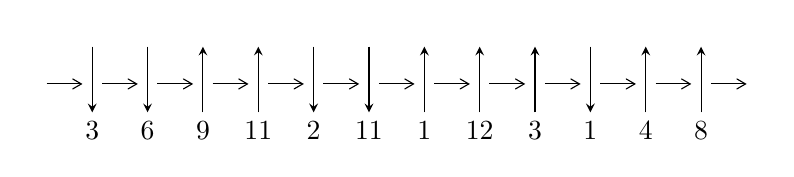
\begin{tikzpicture}[x=20pt, y=17pt]
	% nodes
	\node (C0) at (0, 0) {};
	\node (C1) at (1, 0) {};
	\node (C1U) at (1, +1) {};
	\node (C1D) at (1, -1) {3};

	\node (C2) at (2, 0) {};
	\node (C2U) at (2, +1) {};
	\node (C2D) at (2, -1) {6};

	\node (C3) at (3, 0) {};
	\node (C3U) at (3, +1) {};
	\node (C3D) at (3, -1) {9};

	\node (C4) at (4, 0) {};
	\node (C4U) at (4, +1) {};
	\node (C4D) at (4, -1) {11};

	\node (C5) at (5, 0) {};
	\node (C5U) at (5, +1) {};
	\node (C5D) at (5, -1) {2};

	\node (C6) at (6, 0) {};
	\node (C6U) at (6, +1) {};
	\node (C6D) at (6, -1) {11};

	\node (C7) at (7, 0) {};
	\node (C7U) at (7, +1) {};
	\node (C7D) at (7, -1) {1};

	\node (C8) at (8, 0) {};
	\node (C8U) at (8, +1) {};
	\node (C8D) at (8, -1) {12};

	\node (C9) at (9, 0) {};
	\node (C9U) at (9, +1) {};
	\node (C9D) at (9, -1) {3};

	\node (C10) at (10, 0) {};
	\node (C10U) at (10, +1) {};
	\node (C10D) at (10, -1) {1};

	\node (C11) at (11, 0) {};
	\node (C11U) at (11, +1) {};
	\node (C11D) at (11, -1) {4};

	\node (C12) at (12, 0) {};
	\node (C12U) at (12, +1) {};
	\node (C12D) at (12, -1) {8};
	\node (C13) at (13, 0) {};

	% arrows
	\draw[->,>={angle 60}]
	(C0) edge (C1) (C1) edge (C2) (C2) edge (C3) (C3) edge (C4) (C4) edge (C5) (C5) edge (C6) (C6) edge (C7) (C7) edge (C8) (C8) edge (C9) (C9) edge (C10) (C10) edge (C11) (C11) edge (C12) (C12) edge (C13) ;	\draw[->,>=stealth]
	(C1U) edge (C1D) (C2U) edge (C2D) (C3D) edge (C3U) (C4D) edge (C4U) (C5U) edge (C5D) (C6U) edge (C6D) (C7D) edge (C7U) (C8D) edge (C8U) (C9D) edge (C9U) (C10U) edge (C10D) (C11D) edge (C11U) (C12D) edge (C12U) ;
	\end{tikzpicture} \\
\hhline{~~} \\& 
\textbf{Solving Sequence} \\ \cline{2-2} 
 &
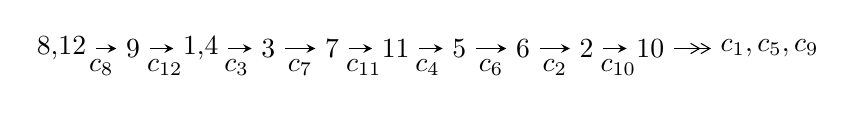
\begin{tikzpicture}[x=23pt, y=7pt]
	% node
	\node (A0) at (-1/8, 0) {8,12};
	\node (A1) at (1, 0) {9};
	\node (A2) at (33/16, 0) {1,4};
	\node (A3) at (25/8, 0) {3};
	\node (A4) at (33/8, 0) {7};
	\node (A5) at (41/8, 0) {11};
	\node (A6) at (49/8, 0) {5};
	\node (A7) at (57/8, 0) {6};
	\node (A8) at (65/8, 0) {2};
	\node (A9) at (73/8, 0) {10};
	\node (C1) at (1/2, -1) {$c_{8}$};
	\node (C2) at (3/2, -1) {$c_{12}$};
	\node (C3) at (21/8, -1) {$c_{3}$};
	\node (C4) at (29/8, -1) {$c_{7}$};
	\node (C5) at (37/8, -1) {$c_{11}$};
	\node (C6) at (45/8, -1) {$c_{4}$};
	\node (C7) at (53/8, -1) {$c_{6}$};
	\node (C8) at (61/8, -1) {$c_{2}$};
	\node (C9) at (69/8, -1) {$c_{10}$};
	\node (A10) at (11, 0) {$c_{1},c_{5},c_{9}$};

	% edge
	\draw[->,>=stealth]	
	(A0) edge (A1) (A1) edge (A2) (A2) edge (A3) (A3) edge (A4) (A4) edge (A5) (A5) edge (A6) (A6) edge (A7) (A7) edge (A8) (A8) edge (A9) ;
	\draw[->>,>={angle 60}]	
	(A9) edge (A10);
\end{tikzpicture} \\ 

\end{tabular} \\

\footnotetext{
The image of knot diagram is generated by the software ``\textbf{Draw programme}" developed by Andrew Bartholomew(\url{http://www.layer8.co.uk/maths/draw/index.htm\#Running-draw}), where we modified some parts for our purpose(\url{https://github.com/CATsTAILs/LinksPainter}).
}\phantom \\ \newline 
\centering \textbf{Ideals for irreducible components\footnotemark of $X_{\text{par}}$} 
 
\begin{align*}
I^u_{1}&=\langle 
3 u^{25}+33 u^{24}+\cdots+4 b+36,\;17 u^{25}+196 u^{24}+\cdots+32 a+656,\;u^{26}+12 u^{25}+\cdots+288 u+32\rangle \\
I^u_{2}&=\langle 
-333638458 a^9 u^2+2803980318 a^8 u^2+\cdots-878011078 a-1380422771,\\
\phantom{I^u_{2}}&\phantom{= \langle  }a^9 u^2+5 a^8 u^2+\cdots+528 a+584,\;u^3- u^2+2 u-1\rangle \\
I^u_{3}&=\langle 
2 u^{17}+15 u^{15}+\cdots+b+2,\;2 u^{16}-2 u^{15}+\cdots+a+4,\;u^{18}- u^{17}+\cdots-4 u+1\rangle \\
\\
\end{align*}
\raggedright * 3 irreducible components of $\dim_{\mathbb{C}}=0$, with total 74 representations.\\
\footnotetext{All coefficients of polynomials are rational numbers. But the coefficients are sometimes approximated in decimal forms when there is not enough margin.}
\newpage
\renewcommand{\arraystretch}{1}
\centering \section*{I. $I^u_{1}= \langle 3 u^{25}+33 u^{24}+\cdots+4 b+36,\;17 u^{25}+196 u^{24}+\cdots+32 a+656,\;u^{26}+12 u^{25}+\cdots+288 u+32 \rangle$}
\flushleft \textbf{(i) Arc colorings}\\
\begin{tabular}{m{7pt} m{180pt} m{7pt} m{180pt} }
\flushright $a_{8}=$&$\begin{pmatrix}1\\0\end{pmatrix}$ \\
\flushright $a_{12}=$&$\begin{pmatrix}0\\u\end{pmatrix}$ \\
\flushright $a_{9}=$&$\begin{pmatrix}1\\- u^2\end{pmatrix}$ \\
\flushright $a_{1}=$&$\begin{pmatrix}u\\u\end{pmatrix}$ \\
\flushright $a_{4}=$&$\begin{pmatrix}-0.531250 u^{25}-6.12500 u^{24}+\cdots-148.500 u-20.5000\\-\frac{3}{4} u^{25}-\frac{33}{4} u^{24}+\cdots-\frac{155}{2} u-9\end{pmatrix}$ \\
\flushright $a_{3}=$&$\begin{pmatrix}-\frac{9}{32} u^{25}-\frac{21}{8} u^{24}+\cdots-16 u-\frac{7}{2}\\\frac{1}{2} u^{25}+\frac{23}{4} u^{24}+\cdots+\frac{149}{2} u+7\end{pmatrix}$ \\
\flushright $a_{7}=$&$\begin{pmatrix}u^2+1\\u^2\end{pmatrix}$ \\
\flushright $a_{11}=$&$\begin{pmatrix}-\frac{19}{32} u^{25}-\frac{105}{16} u^{24}+\cdots-134 u-16\\-\frac{3}{16} u^{25}-\frac{17}{8} u^{24}+\cdots-11 u-1\end{pmatrix}$ \\
\flushright $a_{5}=$&$\begin{pmatrix}2.87500 u^{25}+30.5625 u^{24}+\cdots+671.750 u+82.5000\\-\frac{23}{16} u^{25}-\frac{137}{8} u^{24}+\cdots-\frac{483}{2} u-26\end{pmatrix}$ \\
\flushright $a_{6}=$&$\begin{pmatrix}-\frac{57}{32} u^{25}-\frac{157}{8} u^{24}+\cdots-\frac{1077}{2} u-68\\\frac{3}{4} u^{25}+\frac{69}{8} u^{24}+\cdots+116 u+13\end{pmatrix}$ \\
\flushright $a_{2}=$&$\begin{pmatrix}-\frac{1}{32} u^{25}-\frac{3}{16} u^{24}+\cdots+23 u+3\\\frac{9}{16} u^{25}+\frac{51}{8} u^{24}+\cdots+155 u+19\end{pmatrix}$ \\
\flushright $a_{10}=$&$\begin{pmatrix}\frac{1}{32} u^{25}+\frac{3}{16} u^{24}+\cdots-21 u-2\\\frac{7}{16} u^{25}+\frac{37}{8} u^{24}+\cdots+102 u+13\end{pmatrix}$\\&\end{tabular}
\flushleft \textbf{(ii) Obstruction class $= -1$}\\~\\
\flushleft \textbf{(iii) Cusp Shapes $= -\frac{7}{4} u^{25}-20 u^{24}+\cdots-292 u-18$}\\~\\
\newpage\renewcommand{\arraystretch}{1}
\flushleft \textbf{(iv) u-Polynomials at the component}\newline \\
\begin{tabular}{m{50pt}|m{274pt}}
Crossings & \hspace{64pt}u-Polynomials at each crossing \\
\hline $$\begin{aligned}c_{1}\end{aligned}$$&$\begin{aligned}
&u^{26}+9 u^{25}+\cdots+96 u+64
\end{aligned}$\\
\hline $$\begin{aligned}c_{2},c_{5}\end{aligned}$$&$\begin{aligned}
&u^{26}+9 u^{25}+\cdots+24 u+8
\end{aligned}$\\
\hline $$\begin{aligned}c_{3},c_{4},c_{9}\\c_{11}\end{aligned}$$&$\begin{aligned}
&u^{26}+8 u^{24}+\cdots+3 u+1
\end{aligned}$\\
\hline $$\begin{aligned}c_{6},c_{10}\end{aligned}$$&$\begin{aligned}
&u^{26}+u^{25}+\cdots+14 u+1
\end{aligned}$\\
\hline $$\begin{aligned}c_{7},c_{8},c_{12}\end{aligned}$$&$\begin{aligned}
&u^{26}-12 u^{25}+\cdots-288 u+32
\end{aligned}$\\
\hline
\end{tabular}\\~\\
\newpage\renewcommand{\arraystretch}{1}
\flushleft \textbf{(v) Riley Polynomials at the component}\newline \\
\begin{tabular}{m{50pt}|m{274pt}}
Crossings & \hspace{64pt}Riley Polynomials at each crossing \\
\hline $$\begin{aligned}c_{1}\end{aligned}$$&$\begin{aligned}
&y^{26}+19 y^{25}+\cdots-8704 y+4096
\end{aligned}$\\
\hline $$\begin{aligned}c_{2},c_{5}\end{aligned}$$&$\begin{aligned}
&y^{26}-9 y^{25}+\cdots-96 y+64
\end{aligned}$\\
\hline $$\begin{aligned}c_{3},c_{4},c_{9}\\c_{11}\end{aligned}$$&$\begin{aligned}
&y^{26}+16 y^{25}+\cdots+5 y+1
\end{aligned}$\\
\hline $$\begin{aligned}c_{6},c_{10}\end{aligned}$$&$\begin{aligned}
&y^{26}+39 y^{25}+\cdots-50 y+1
\end{aligned}$\\
\hline $$\begin{aligned}c_{7},c_{8},c_{12}\end{aligned}$$&$\begin{aligned}
&y^{26}+22 y^{25}+\cdots+512 y+1024
\end{aligned}$\\
\hline
\end{tabular}\\~\\
\newpage\flushleft \textbf{(vi) Complex Volumes and Cusp Shapes}
$$\begin{array}{c|c|c}  
\text{Solutions to }I^u_{1}& \I (\text{vol} + \sqrt{-1}CS) & \text{Cusp shape}\\
 \hline 
\begin{aligned}
u &= -0.373580 + 0.933614 I \\
a &= \phantom{-}0.280319 + 0.410765 I \\
b &= \phantom{-}0.406899 + 0.387993 I\end{aligned}
 & -0.83502 - 2.62007 I & \phantom{-}5.29205 + 6.35608 I \\ \hline\begin{aligned}
u &= -0.373580 - 0.933614 I \\
a &= \phantom{-}0.280319 - 0.410765 I \\
b &= \phantom{-}0.406899 - 0.387993 I\end{aligned}
 & -0.83502 + 2.62007 I & \phantom{-}5.29205 - 6.35608 I \\ \hline\begin{aligned}
u &= -0.977022 + 0.289560 I \\
a &= -0.999855 + 0.807238 I \\
b &= -0.329282 - 0.190408 I\end{aligned}
 & \phantom{-}5.86673 - 2.98457 I & \phantom{-}2.91733 + 2.32225 I \\ \hline\begin{aligned}
u &= -0.977022 - 0.289560 I \\
a &= -0.999855 - 0.807238 I \\
b &= -0.329282 + 0.190408 I\end{aligned}
 & \phantom{-}5.86673 + 2.98457 I & \phantom{-}2.91733 - 2.32225 I \\ \hline\begin{aligned}
u &= -1.040460 + 0.290353 I \\
a &= \phantom{-}0.885056 - 0.906575 I \\
b &= \phantom{-}0.321883 + 0.239511 I\end{aligned}
 & \phantom{-}4.93150 - 9.47568 I & \phantom{-}1.22997 + 6.65192 I \\ \hline\begin{aligned}
u &= -1.040460 - 0.290353 I \\
a &= \phantom{-}0.885056 + 0.906575 I \\
b &= \phantom{-}0.321883 - 0.239511 I\end{aligned}
 & \phantom{-}4.93150 + 9.47568 I & \phantom{-}1.22997 - 6.65192 I \\ \hline\begin{aligned}
u &= -0.893372 + 0.672431 I \\
a &= \phantom{-}0.616422 - 0.459995 I \\
b &= \phantom{-}0.580795 + 0.074295 I\end{aligned}
 & -1.98248 - 3.07677 I & -3.82004 + 5.96476 I \\ \hline\begin{aligned}
u &= -0.893372 - 0.672431 I \\
a &= \phantom{-}0.616422 + 0.459995 I \\
b &= \phantom{-}0.580795 - 0.074295 I\end{aligned}
 & -1.98248 + 3.07677 I & -3.82004 - 5.96476 I \\ \hline\begin{aligned}
u &= -0.658604 + 1.099520 I \\
a &= -0.357985 + 0.662624 I \\
b &= -0.744381 + 0.825205 I\end{aligned}
 & \phantom{-}3.47939 - 2.75359 I & \phantom{-0.000000 -}0. + 1.54097 I \\ \hline\begin{aligned}
u &= -0.658604 - 1.099520 I \\
a &= -0.357985 - 0.662624 I \\
b &= -0.744381 - 0.825205 I\end{aligned}
 & \phantom{-}3.47939 + 2.75359 I & \phantom{-0.000000 } 0. - 1.54097 I\\
 \hline 
 \end{array}$$\newpage$$\begin{array}{c|c|c}  
\text{Solutions to }I^u_{1}& \I (\text{vol} + \sqrt{-1}CS) & \text{Cusp shape}\\
 \hline 
\begin{aligned}
u &= -0.737527 + 1.134930 I \\
a &= \phantom{-}0.473155 - 0.623862 I \\
b &= \phantom{-}1.037410 - 0.669242 I\end{aligned}
 & \phantom{-}2.46178 + 3.30067 I & -1.81816 - 2.93564 I \\ \hline\begin{aligned}
u &= -0.737527 - 1.134930 I \\
a &= \phantom{-}0.473155 + 0.623862 I \\
b &= \phantom{-}1.037410 + 0.669242 I\end{aligned}
 & \phantom{-}2.46178 - 3.30067 I & -1.81816 + 2.93564 I \\ \hline\begin{aligned}
u &= -0.500184 + 0.273597 I \\
a &= -1.113850 + 0.000222 I \\
b &= -0.361841 - 0.000040 I\end{aligned}
 & \phantom{-}1.011870 - 0.620695 I & \phantom{-}7.41936 + 3.02549 I \\ \hline\begin{aligned}
u &= -0.500184 - 0.273597 I \\
a &= -1.113850 - 0.000222 I \\
b &= -0.361841 + 0.000040 I\end{aligned}
 & \phantom{-}1.011870 + 0.620695 I & \phantom{-}7.41936 - 3.02549 I \\ \hline\begin{aligned}
u &= \phantom{-}0.345460 + 0.396654 I \\
a &= \phantom{-}0.416298 + 0.809635 I \\
b &= \phantom{-}0.415031 - 0.528152 I\end{aligned}
 & -1.54818 + 1.01569 I & -2.49851 + 1.48185 I \\ \hline\begin{aligned}
u &= \phantom{-}0.345460 - 0.396654 I \\
a &= \phantom{-}0.416298 - 0.809635 I \\
b &= \phantom{-}0.415031 + 0.528152 I\end{aligned}
 & -1.54818 - 1.01569 I & -2.49851 - 1.48185 I \\ \hline\begin{aligned}
u &= -0.12954 + 1.47954 I \\
a &= \phantom{-}0.663655 + 0.382952 I \\
b &= \phantom{-}1.94741 + 0.15396 I\end{aligned}
 & -4.82392 - 2.67431 I & \phantom{-0.000000 } 0 \\ \hline\begin{aligned}
u &= -0.12954 - 1.47954 I \\
a &= \phantom{-}0.663655 - 0.382952 I \\
b &= \phantom{-}1.94741 - 0.15396 I\end{aligned}
 & -4.82392 + 2.67431 I & \phantom{-0.000000 } 0 \\ \hline\begin{aligned}
u &= -0.39186 + 1.47047 I \\
a &= \phantom{-}1.031950 + 0.307632 I \\
b &= \phantom{-}2.57514 + 0.41031 I\end{aligned}
 & \phantom{-}0.23550 - 7.89653 I & \phantom{-0.000000 } 0 \\ \hline\begin{aligned}
u &= -0.39186 - 1.47047 I \\
a &= \phantom{-}1.031950 - 0.307632 I \\
b &= \phantom{-}2.57514 - 0.41031 I\end{aligned}
 & \phantom{-}0.23550 + 7.89653 I & \phantom{-0.000000 } 0\\
 \hline 
 \end{array}$$\newpage$$\begin{array}{c|c|c}  
\text{Solutions to }I^u_{1}& \I (\text{vol} + \sqrt{-1}CS) & \text{Cusp shape}\\
 \hline 
\begin{aligned}
u &= -0.42139 + 1.47806 I \\
a &= -1.077660 - 0.235946 I \\
b &= -2.67192 - 0.32255 I\end{aligned}
 & -0.7052 - 14.6997 I & \phantom{-0.000000 -}0. + 7.55199 I \\ \hline\begin{aligned}
u &= -0.42139 - 1.47806 I \\
a &= -1.077660 + 0.235946 I \\
b &= -2.67192 + 0.32255 I\end{aligned}
 & -0.7052 + 14.6997 I & \phantom{-0.000000 } 0. - 7.55199 I \\ \hline\begin{aligned}
u &= \phantom{-}0.04653 + 1.56180 I \\
a &= -0.561335 - 0.336020 I \\
b &= -1.91553 + 0.15501 I\end{aligned}
 & -8.47892 + 2.46726 I & \phantom{-0.000000 } 0 \\ \hline\begin{aligned}
u &= \phantom{-}0.04653 - 1.56180 I \\
a &= -0.561335 + 0.336020 I \\
b &= -1.91553 - 0.15501 I\end{aligned}
 & -8.47892 - 2.46726 I & \phantom{-0.000000 } 0 \\ \hline\begin{aligned}
u &= -0.26846 + 1.59618 I \\
a &= -0.756170 - 0.252389 I \\
b &= -2.26161 - 0.13367 I\end{aligned}
 & -9.48266 - 7.26585 I & \phantom{-0.000000 } 0 \\ \hline\begin{aligned}
u &= -0.26846 - 1.59618 I \\
a &= -0.756170 + 0.252389 I \\
b &= -2.26161 + 0.13367 I\end{aligned}
 & -9.48266 + 7.26585 I & \phantom{-0.000000 } 0\\
 \hline 
 \end{array}$$\newpage\newpage\renewcommand{\arraystretch}{1}
\centering \section*{II. $I^u_{2}= \langle -3.34\times10^{8} a^{9} u^{2}+2.80\times10^{9} a^{8} u^{2}+\cdots-8.78\times10^{8} a-1.38\times10^{9},\;a^9 u^2+5 a^8 u^2+\cdots+528 a+584,\;u^3- u^2+2 u-1 \rangle$}
\flushleft \textbf{(i) Arc colorings}\\
\begin{tabular}{m{7pt} m{180pt} m{7pt} m{180pt} }
\flushright $a_{8}=$&$\begin{pmatrix}1\\0\end{pmatrix}$ \\
\flushright $a_{12}=$&$\begin{pmatrix}0\\u\end{pmatrix}$ \\
\flushright $a_{9}=$&$\begin{pmatrix}1\\- u^2\end{pmatrix}$ \\
\flushright $a_{1}=$&$\begin{pmatrix}u\\u\end{pmatrix}$ \\
\flushright $a_{4}=$&$\begin{pmatrix}a\\0.209620 a^{9} u^{2}-1.76170 a^{8} u^{2}+\cdots+0.551640 a+0.867297\end{pmatrix}$ \\
\flushright $a_{3}=$&$\begin{pmatrix}-0.209620 a^{9} u^{2}+1.76170 a^{8} u^{2}+\cdots+0.448360 a-0.867297\\-1.52915 a^{9} u^{2}+2.83867 a^{8} u^{2}+\cdots+1.28335 a+1.54825\end{pmatrix}$ \\
\flushright $a_{7}=$&$\begin{pmatrix}u^2+1\\u^2\end{pmatrix}$ \\
\flushright $a_{11}=$&$\begin{pmatrix}- a^2 u\\-1.83712 a^{9} u^{2}+2.43089 a^{8} u^{2}+\cdots-0.217188 a+3.13850\end{pmatrix}$ \\
\flushright $a_{5}=$&$\begin{pmatrix}a^3 u^2+a\\-2.20070 a^{9} u^{2}+2.46990 a^{8} u^{2}+\cdots-1.35859 a+2.49562\end{pmatrix}$ \\
\flushright $a_{6}=$&$\begin{pmatrix}1.87891 a^{9} u^{2}-3.01206 a^{8} u^{2}+\cdots-0.212937 a-1.75521\\2.51980 a^{9} u^{2}-2.23306 a^{8} u^{2}+\cdots+1.62064 a-2.93193\end{pmatrix}$ \\
\flushright $a_{2}=$&$\begin{pmatrix}-0.232543 a^{9} u^{2}+1.95512 a^{8} u^{2}+\cdots+0.115174 a+0.454433\\- a^2 u^2+2 u-2\end{pmatrix}$ \\
\flushright $a_{10}=$&$\begin{pmatrix}2.70862 a^{9} u^{2}-2.33692 a^{8} u^{2}+\cdots+1.65477 a-1.76434\\0.871503 a^{9} u^{2}+0.0939733 a^{8} u^{2}+\cdots+1.43758 a+1.37417\end{pmatrix}$\\&\end{tabular}
\flushleft \textbf{(ii) Obstruction class $= -1$}\\~\\
\flushleft \textbf{(iii) Cusp Shapes $= \frac{640570216}{1591637129} a^9 u^2+\frac{5775444576}{1591637129} a^8 u^2+\cdots+\frac{12123611228}{1591637129} a+\frac{11646488850}{1591637129}$}\\~\\
\newpage\renewcommand{\arraystretch}{1}
\flushleft \textbf{(iv) u-Polynomials at the component}\newline \\
\begin{tabular}{m{50pt}|m{274pt}}
Crossings & \hspace{64pt}u-Polynomials at each crossing \\
\hline $$\begin{aligned}c_{1}\end{aligned}$$&$\begin{aligned}
&(u^5+u^4+4 u^3+3 u^2+3 u+1)^6
\end{aligned}$\\
\hline $$\begin{aligned}c_{2},c_{5}\end{aligned}$$&$\begin{aligned}
&(u^5- u^4+u^2+u-1)^6
\end{aligned}$\\
\hline $$\begin{aligned}c_{3},c_{4},c_{9}\\c_{11}\end{aligned}$$&$\begin{aligned}
&u^{30}- u^{29}+\cdots+1390 u+773
\end{aligned}$\\
\hline $$\begin{aligned}c_{6},c_{10}\end{aligned}$$&$\begin{aligned}
&u^{30}-3 u^{29}+\cdots-9926 u+2939
\end{aligned}$\\
\hline $$\begin{aligned}c_{7},c_{8},c_{12}\end{aligned}$$&$\begin{aligned}
&(u^3+u^2+2 u+1)^{10}
\end{aligned}$\\
\hline
\end{tabular}\\~\\
\newpage\renewcommand{\arraystretch}{1}
\flushleft \textbf{(v) Riley Polynomials at the component}\newline \\
\begin{tabular}{m{50pt}|m{274pt}}
Crossings & \hspace{64pt}Riley Polynomials at each crossing \\
\hline $$\begin{aligned}c_{1}\end{aligned}$$&$\begin{aligned}
&(y^5+7 y^4+16 y^3+13 y^2+3 y-1)^6
\end{aligned}$\\
\hline $$\begin{aligned}c_{2},c_{5}\end{aligned}$$&$\begin{aligned}
&(y^5- y^4+4 y^3-3 y^2+3 y-1)^6
\end{aligned}$\\
\hline $$\begin{aligned}c_{3},c_{4},c_{9}\\c_{11}\end{aligned}$$&$\begin{aligned}
&y^{30}+15 y^{29}+\cdots+5878292 y+597529
\end{aligned}$\\
\hline $$\begin{aligned}c_{6},c_{10}\end{aligned}$$&$\begin{aligned}
&y^{30}+19 y^{29}+\cdots-67383832 y+8637721
\end{aligned}$\\
\hline $$\begin{aligned}c_{7},c_{8},c_{12}\end{aligned}$$&$\begin{aligned}
&(y^3+3 y^2+2 y-1)^{10}
\end{aligned}$\\
\hline
\end{tabular}\\~\\
\newpage\flushleft \textbf{(vi) Complex Volumes and Cusp Shapes}
$$\begin{array}{c|c|c}  
\text{Solutions to }I^u_{2}& \I (\text{vol} + \sqrt{-1}CS) & \text{Cusp shape}\\
 \hline 
\begin{aligned}
u &= \phantom{-}0.215080 + 1.307140 I \\
a &= -1.014630 + 0.047968 I \\
b &= -2.30589 - 0.97577 I\end{aligned}
 & -8.84111 + 2.82812 I & -11.11859 - 2.97945 I \\ \hline\begin{aligned}
u &= \phantom{-}0.215080 + 1.307140 I \\
a &= \phantom{-}0.771849 - 0.683924 I \\
b &= \phantom{-}1.093870 - 0.106141 I\end{aligned}
 & -6.13913 + 5.04209 I & -2.62407 - 7.20234 I \\ \hline\begin{aligned}
u &= \phantom{-}0.215080 + 1.307140 I \\
a &= -1.115000 - 0.034024 I \\
b &= -2.93266 - 0.29143 I\end{aligned}
 & -6.13913 + 5.04209 I & -2.62407 - 7.20234 I \\ \hline\begin{aligned}
u &= \phantom{-}0.215080 + 1.307140 I \\
a &= -0.784986 + 0.155927 I \\
b &= -2.90073 + 1.14869 I\end{aligned}
 & \phantom{-}2.99936 + 6.15987 I & -1.59102 - 5.34173 I \\ \hline\begin{aligned}
u &= \phantom{-}0.215080 + 1.307140 I \\
a &= \phantom{-}1.217270 + 0.148472 I \\
b &= \phantom{-}2.62933 + 0.23436 I\end{aligned}
 & -6.13913 + 0.61415 I & -2.62407 + 1.24344 I \\ \hline\begin{aligned}
u &= \phantom{-}0.215080 + 1.307140 I \\
a &= \phantom{-}0.305785 + 1.223910 I \\
b &= \phantom{-}0.871169 + 0.998250 I\end{aligned}
 & \phantom{-}2.99936 - 0.50362 I & -1.59102 - 0.61717 I \\ \hline\begin{aligned}
u &= \phantom{-}0.215080 + 1.307140 I \\
a &= \phantom{-}0.683723 - 0.136389 I \\
b &= \phantom{-}2.59396 - 1.27411 I\end{aligned}
 & \phantom{-}2.99936 - 0.50362 I & -1.59102 - 0.61717 I \\ \hline\begin{aligned}
u &= \phantom{-}0.215080 + 1.307140 I \\
a &= -0.127449 - 1.308880 I \\
b &= -0.575167 - 1.111610 I\end{aligned}
 & \phantom{-}2.99936 + 6.15987 I & -1.59102 - 5.34173 I \\ \hline\begin{aligned}
u &= \phantom{-}0.215080 + 1.307140 I \\
a &= \phantom{-}1.290360 - 0.282036 I \\
b &= \phantom{-}2.26738 + 0.12156 I\end{aligned}
 & -8.84111 + 2.82812 I & -11.11859 - 2.97945 I \\ \hline\begin{aligned}
u &= \phantom{-}0.215080 + 1.307140 I \\
a &= -0.564558 + 0.306692 I \\
b &= -0.833786 - 0.795800 I\end{aligned}
 & -6.13913 + 0.61415 I & -2.62407 + 1.24344 I\\
 \hline 
 \end{array}$$\newpage$$\begin{array}{c|c|c}  
\text{Solutions to }I^u_{2}& \I (\text{vol} + \sqrt{-1}CS) & \text{Cusp shape}\\
 \hline 
\begin{aligned}
u &= \phantom{-}0.215080 - 1.307140 I \\
a &= -1.014630 - 0.047968 I \\
b &= -2.30589 + 0.97577 I\end{aligned}
 & -8.84111 - 2.82812 I & -11.11859 + 2.97945 I \\ \hline\begin{aligned}
u &= \phantom{-}0.215080 - 1.307140 I \\
a &= \phantom{-}0.771849 + 0.683924 I \\
b &= \phantom{-}1.093870 + 0.106141 I\end{aligned}
 & -6.13913 - 5.04209 I & -2.62407 + 7.20234 I \\ \hline\begin{aligned}
u &= \phantom{-}0.215080 - 1.307140 I \\
a &= -1.115000 + 0.034024 I \\
b &= -2.93266 + 0.29143 I\end{aligned}
 & -6.13913 - 5.04209 I & -2.62407 + 7.20234 I \\ \hline\begin{aligned}
u &= \phantom{-}0.215080 - 1.307140 I \\
a &= -0.784986 - 0.155927 I \\
b &= -2.90073 - 1.14869 I\end{aligned}
 & \phantom{-}2.99936 - 6.15987 I & -1.59102 + 5.34173 I \\ \hline\begin{aligned}
u &= \phantom{-}0.215080 - 1.307140 I \\
a &= \phantom{-}1.217270 - 0.148472 I \\
b &= \phantom{-}2.62933 - 0.23436 I\end{aligned}
 & -6.13913 - 0.61415 I & -2.62407 - 1.24344 I \\ \hline\begin{aligned}
u &= \phantom{-}0.215080 - 1.307140 I \\
a &= \phantom{-}0.305785 - 1.223910 I \\
b &= \phantom{-}0.871169 - 0.998250 I\end{aligned}
 & \phantom{-}2.99936 + 0.50362 I & -1.59102 + 0.61717 I \\ \hline\begin{aligned}
u &= \phantom{-}0.215080 - 1.307140 I \\
a &= \phantom{-}0.683723 + 0.136389 I \\
b &= \phantom{-}2.59396 + 1.27411 I\end{aligned}
 & \phantom{-}2.99936 + 0.50362 I & -1.59102 + 0.61717 I \\ \hline\begin{aligned}
u &= \phantom{-}0.215080 - 1.307140 I \\
a &= -0.127449 + 1.308880 I \\
b &= -0.575167 + 1.111610 I\end{aligned}
 & \phantom{-}2.99936 - 6.15987 I & -1.59102 + 5.34173 I \\ \hline\begin{aligned}
u &= \phantom{-}0.215080 - 1.307140 I \\
a &= \phantom{-}1.290360 + 0.282036 I \\
b &= \phantom{-}2.26738 - 0.12156 I\end{aligned}
 & -8.84111 - 2.82812 I & -11.11859 + 2.97945 I \\ \hline\begin{aligned}
u &= \phantom{-}0.215080 - 1.307140 I \\
a &= -0.564558 - 0.306692 I \\
b &= -0.833786 + 0.795800 I\end{aligned}
 & -6.13913 - 0.61415 I & -2.62407 - 1.24344 I\\
 \hline 
 \end{array}$$\newpage$$\begin{array}{c|c|c}  
\text{Solutions to }I^u_{2}& \I (\text{vol} + \sqrt{-1}CS) & \text{Cusp shape}\\
 \hline 
\begin{aligned}
u &= \phantom{-}0.569840\phantom{ +0.000000I} \\
a &= -0.494172 + 1.023630 I \\
b &= \phantom{-}0.055265 + 0.919402 I\end{aligned}
 & -2.00154 - 2.21397 I & \phantom{-}3.90519 + 4.22289 I \\ \hline\begin{aligned}
u &= \phantom{-}0.569840\phantom{ +0.000000I} \\
a &= -0.494172 - 1.023630 I \\
b &= \phantom{-}0.055265 - 0.919402 I\end{aligned}
 & -2.00154 + 2.21397 I & \phantom{-}3.90519 - 4.22289 I \\ \hline\begin{aligned}
u &= \phantom{-}0.569840\phantom{ +0.000000I} \\
a &= -1.81678 + 0.97410 I \\
b &= -0.401412 - 1.037940 I\end{aligned}
 & \phantom{-}7.13694 + 3.33174 I & \phantom{-}4.93825 - 2.36228 I \\ \hline\begin{aligned}
u &= \phantom{-}0.569840\phantom{ +0.000000I} \\
a &= -1.81678 - 0.97410 I \\
b &= -0.401412 + 1.037940 I\end{aligned}
 & \phantom{-}7.13694 - 3.33174 I & \phantom{-}4.93825 + 2.36228 I \\ \hline\begin{aligned}
u &= \phantom{-}0.569840\phantom{ +0.000000I} \\
a &= \phantom{-}1.73970 + 1.26637 I \\
b &= \phantom{-}0.470359 - 0.966293 I\end{aligned}
 & \phantom{-}7.13694 + 3.33174 I & \phantom{-}4.93825 - 2.36228 I \\ \hline\begin{aligned}
u &= \phantom{-}0.569840\phantom{ +0.000000I} \\
a &= \phantom{-}1.73970 - 1.26637 I \\
b &= \phantom{-}0.470359 + 0.966293 I\end{aligned}
 & \phantom{-}7.13694 - 3.33174 I & \phantom{-}4.93825 + 2.36228 I \\ \hline\begin{aligned}
u &= \phantom{-}0.569840\phantom{ +0.000000I} \\
a &= \phantom{-}0.18462 + 2.19674 I \\
b &= \phantom{-}0.221651 - 0.130016 I\end{aligned}
 & -2.00154 + 2.21397 I & \phantom{-}3.90519 - 4.22289 I \\ \hline\begin{aligned}
u &= \phantom{-}0.569840\phantom{ +0.000000I} \\
a &= \phantom{-}0.18462 - 2.19674 I \\
b &= \phantom{-}0.221651 + 0.130016 I\end{aligned}
 & -2.00154 - 2.21397 I & \phantom{-}3.90519 + 4.22289 I \\ \hline\begin{aligned}
u &= \phantom{-}0.569840\phantom{ +0.000000I} \\
a &= -0.27573 + 2.20498 I \\
b &= \phantom{-}0.246656 + 0.540491 I\end{aligned}
 & -4.70353\phantom{ +0.000000I} & -4.58932 + 0. I\phantom{ +0.000000I} \\ \hline\begin{aligned}
u &= \phantom{-}0.569840\phantom{ +0.000000I} \\
a &= -0.27573 - 2.20498 I \\
b &= \phantom{-}0.246656 - 0.540491 I\end{aligned}
 & -4.70353\phantom{ +0.000000I} & -4.58932 + 0. I\phantom{ +0.000000I}\\
 \hline 
 \end{array}$$\newpage\newpage\renewcommand{\arraystretch}{1}
\centering \section*{III. $I^u_{3}= \langle 2 u^{17}+15 u^{15}+\cdots+b+2,\;2 u^{16}-2 u^{15}+\cdots+a+4,\;u^{18}- u^{17}+\cdots-4 u+1 \rangle$}
\flushleft \textbf{(i) Arc colorings}\\
\begin{tabular}{m{7pt} m{180pt} m{7pt} m{180pt} }
\flushright $a_{8}=$&$\begin{pmatrix}1\\0\end{pmatrix}$ \\
\flushright $a_{12}=$&$\begin{pmatrix}0\\u\end{pmatrix}$ \\
\flushright $a_{9}=$&$\begin{pmatrix}1\\- u^2\end{pmatrix}$ \\
\flushright $a_{1}=$&$\begin{pmatrix}u\\u\end{pmatrix}$ \\
\flushright $a_{4}=$&$\begin{pmatrix}-2 u^{16}+2 u^{15}+\cdots-4 u-4\\-2 u^{17}-15 u^{15}+\cdots+4 u-2\end{pmatrix}$ \\
\flushright $a_{3}=$&$\begin{pmatrix}2 u^{17}-4 u^{16}+\cdots-21 u^2-4\\-3 u^{16}+4 u^{15}+\cdots+6 u-2\end{pmatrix}$ \\
\flushright $a_{7}=$&$\begin{pmatrix}u^2+1\\u^2\end{pmatrix}$ \\
\flushright $a_{11}=$&$\begin{pmatrix}-2 u^{17}+2 u^{16}+\cdots-22 u+5\\- u^{17}+2 u^{16}+\cdots-4 u+2\end{pmatrix}$ \\
\flushright $a_{5}=$&$\begin{pmatrix}u^{17}-3 u^{16}+\cdots+13 u-2\\-3 u^{17}-21 u^{15}+\cdots+19 u-5\end{pmatrix}$ \\
\flushright $a_{6}=$&$\begin{pmatrix}u^{17}-2 u^{16}+\cdots+27 u-5\\-2 u^{17}+u^{16}+\cdots+6 u-3\end{pmatrix}$ \\
\flushright $a_{2}=$&$\begin{pmatrix}- u^{16}-8 u^{14}+\cdots-15 u+1\\- u^{16}+u^{15}+\cdots-19 u^2+3 u\end{pmatrix}$ \\
\flushright $a_{10}=$&$\begin{pmatrix}-2 u^{17}+u^{16}+\cdots-19 u+4\\- u^{17}+u^{16}+\cdots- u+1\end{pmatrix}$\\&\end{tabular}
\flushleft \textbf{(ii) Obstruction class $= 1$}\\~\\
\flushleft \textbf{(iii) Cusp Shapes $= -2 u^{17}+7 u^{16}-24 u^{15}+61 u^{14}-112 u^{13}+219 u^{12}-282 u^{11}+425 u^{10}-445 u^9+493 u^8-466 u^7+358 u^6-299 u^5+167 u^4-81 u^3+44 u^2+7 u-5$}\\~\\
\newpage\renewcommand{\arraystretch}{1}
\flushleft \textbf{(iv) u-Polynomials at the component}\newline \\
\begin{tabular}{m{50pt}|m{274pt}}
Crossings & \hspace{64pt}u-Polynomials at each crossing \\
\hline $$\begin{aligned}c_{1}\end{aligned}$$&$\begin{aligned}
&u^{18}-8 u^{17}+\cdots-8 u+1
\end{aligned}$\\
\hline $$\begin{aligned}c_{2}\end{aligned}$$&$\begin{aligned}
&u^{18}+2 u^{17}+\cdots+2 u+1
\end{aligned}$\\
\hline $$\begin{aligned}c_{3},c_{11}\end{aligned}$$&$\begin{aligned}
&u^{18}+7 u^{16}+\cdots+13 u^2+1
\end{aligned}$\\
\hline $$\begin{aligned}c_{4},c_{9}\end{aligned}$$&$\begin{aligned}
&u^{18}+7 u^{16}+\cdots+13 u^2+1
\end{aligned}$\\
\hline $$\begin{aligned}c_{5}\end{aligned}$$&$\begin{aligned}
&u^{18}-2 u^{17}+\cdots-2 u+1
\end{aligned}$\\
\hline $$\begin{aligned}c_{6},c_{10}\end{aligned}$$&$\begin{aligned}
&u^{18}+u^{17}+\cdots+u+1
\end{aligned}$\\
\hline $$\begin{aligned}c_{7},c_{8}\end{aligned}$$&$\begin{aligned}
&u^{18}- u^{17}+\cdots-4 u+1
\end{aligned}$\\
\hline $$\begin{aligned}c_{12}\end{aligned}$$&$\begin{aligned}
&u^{18}+u^{17}+\cdots+4 u+1
\end{aligned}$\\
\hline
\end{tabular}\\~\\
\newpage\renewcommand{\arraystretch}{1}
\flushleft \textbf{(v) Riley Polynomials at the component}\newline \\
\begin{tabular}{m{50pt}|m{274pt}}
Crossings & \hspace{64pt}Riley Polynomials at each crossing \\
\hline $$\begin{aligned}c_{1}\end{aligned}$$&$\begin{aligned}
&y^{18}+12 y^{17}+\cdots+16 y+1
\end{aligned}$\\
\hline $$\begin{aligned}c_{2},c_{5}\end{aligned}$$&$\begin{aligned}
&y^{18}-8 y^{17}+\cdots-8 y+1
\end{aligned}$\\
\hline $$\begin{aligned}c_{3},c_{4},c_{9}\\c_{11}\end{aligned}$$&$\begin{aligned}
&y^{18}+14 y^{17}+\cdots+26 y+1
\end{aligned}$\\
\hline $$\begin{aligned}c_{6},c_{10}\end{aligned}$$&$\begin{aligned}
&y^{18}+5 y^{17}+\cdots-9 y+1
\end{aligned}$\\
\hline $$\begin{aligned}c_{7},c_{8},c_{12}\end{aligned}$$&$\begin{aligned}
&y^{18}+19 y^{17}+\cdots+26 y+1
\end{aligned}$\\
\hline
\end{tabular}\\~\\
\newpage\flushleft \textbf{(vi) Complex Volumes and Cusp Shapes}
$$\begin{array}{c|c|c}  
\text{Solutions to }I^u_{3}& \I (\text{vol} + \sqrt{-1}CS) & \text{Cusp shape}\\
 \hline 
\begin{aligned}
u &= -0.548156 + 0.847238 I \\
a &= -0.223507 + 0.171449 I \\
b &= -0.275267 - 0.419395 I\end{aligned}
 & -1.41562 - 2.18118 I & -2.40356 + 0.24504 I \\ \hline\begin{aligned}
u &= -0.548156 - 0.847238 I \\
a &= -0.223507 - 0.171449 I \\
b &= -0.275267 + 0.419395 I\end{aligned}
 & -1.41562 + 2.18118 I & -2.40356 - 0.24504 I \\ \hline\begin{aligned}
u &= -0.289325 + 0.967313 I \\
a &= -0.214015 - 0.827701 I \\
b &= \phantom{-}1.143520 - 0.792525 I\end{aligned}
 & \phantom{-}4.75616 - 4.41472 I & \phantom{-}1.35648 + 3.62940 I \\ \hline\begin{aligned}
u &= -0.289325 - 0.967313 I \\
a &= -0.214015 + 0.827701 I \\
b &= \phantom{-}1.143520 + 0.792525 I\end{aligned}
 & \phantom{-}4.75616 + 4.41472 I & \phantom{-}1.35648 - 3.62940 I \\ \hline\begin{aligned}
u &= -0.301562 + 1.039980 I \\
a &= -0.015170 + 0.829040 I \\
b &= -1.39264 + 0.54596 I\end{aligned}
 & \phantom{-}4.48430 + 2.10133 I & \phantom{-}1.59454 - 2.04993 I \\ \hline\begin{aligned}
u &= -0.301562 - 1.039980 I \\
a &= -0.015170 - 0.829040 I \\
b &= -1.39264 - 0.54596 I\end{aligned}
 & \phantom{-}4.48430 - 2.10133 I & \phantom{-}1.59454 + 2.04993 I \\ \hline\begin{aligned}
u &= \phantom{-}0.826816 + 0.217598 I \\
a &= -0.35619 - 1.39245 I \\
b &= -0.265916 - 0.214656 I\end{aligned}
 & -4.52038 + 1.43762 I & -3.35124 - 4.60330 I \\ \hline\begin{aligned}
u &= \phantom{-}0.826816 - 0.217598 I \\
a &= -0.35619 + 1.39245 I \\
b &= -0.265916 + 0.214656 I\end{aligned}
 & -4.52038 - 1.43762 I & -3.35124 + 4.60330 I \\ \hline\begin{aligned}
u &= \phantom{-}0.278515 + 1.287490 I \\
a &= -1.123880 + 0.058895 I \\
b &= -2.12241 - 0.53151 I\end{aligned}
 & -7.92752 + 2.43301 I & -1.35565 + 0.52411 I \\ \hline\begin{aligned}
u &= \phantom{-}0.278515 - 1.287490 I \\
a &= -1.123880 - 0.058895 I \\
b &= -2.12241 + 0.53151 I\end{aligned}
 & -7.92752 - 2.43301 I & -1.35565 - 0.52411 I\\
 \hline 
 \end{array}$$\newpage$$\begin{array}{c|c|c}  
\text{Solutions to }I^u_{3}& \I (\text{vol} + \sqrt{-1}CS) & \text{Cusp shape}\\
 \hline 
\begin{aligned}
u &= \phantom{-}0.094154 + 1.349150 I \\
a &= -0.996965 + 0.368074 I \\
b &= -2.30279 - 0.39041 I\end{aligned}
 & -7.09698 + 2.98270 I & -3.08593 - 3.04995 I \\ \hline\begin{aligned}
u &= \phantom{-}0.094154 - 1.349150 I \\
a &= -0.996965 - 0.368074 I \\
b &= -2.30279 + 0.39041 I\end{aligned}
 & -7.09698 - 2.98270 I & -3.08593 + 3.04995 I \\ \hline\begin{aligned}
u &= -0.01485 + 1.49543 I \\
a &= \phantom{-}0.746594 - 0.367613 I \\
b &= \phantom{-}2.22443 + 0.33307 I\end{aligned}
 & -9.34606 - 2.01452 I & -7.23332 - 0.16467 I \\ \hline\begin{aligned}
u &= -0.01485 - 1.49543 I \\
a &= \phantom{-}0.746594 + 0.367613 I \\
b &= \phantom{-}2.22443 - 0.33307 I\end{aligned}
 & -9.34606 + 2.01452 I & -7.23332 + 0.16467 I \\ \hline\begin{aligned}
u &= \phantom{-}0.35110 + 1.52606 I \\
a &= \phantom{-}0.830916 - 0.030800 I \\
b &= \phantom{-}2.13840 + 0.29887 I\end{aligned}
 & -10.29080 + 5.91942 I & -5.83679 - 3.74571 I \\ \hline\begin{aligned}
u &= \phantom{-}0.35110 - 1.52606 I \\
a &= \phantom{-}0.830916 + 0.030800 I \\
b &= \phantom{-}2.13840 - 0.29887 I\end{aligned}
 & -10.29080 - 5.91942 I & -5.83679 + 3.74571 I \\ \hline\begin{aligned}
u &= \phantom{-}0.103300 + 0.232173 I \\
a &= -3.64778 - 2.10197 I \\
b &= -0.147325 - 0.979951 I\end{aligned}
 & -3.18667 - 2.11613 I & -5.18453 + 3.64144 I \\ \hline\begin{aligned}
u &= \phantom{-}0.103300 - 0.232173 I \\
a &= -3.64778 + 2.10197 I \\
b &= -0.147325 + 0.979951 I\end{aligned}
 & -3.18667 + 2.11613 I & -5.18453 - 3.64144 I\\
 \hline 
 \end{array}$$\newpage
\newpage\renewcommand{\arraystretch}{1}
\centering \section*{ IV. u-Polynomials}
\begin{tabular}{m{50pt}|m{274pt}}
Crossings & \hspace{64pt}u-Polynomials at each crossing \\
\hline $$\begin{aligned}c_{1}\end{aligned}$$&$\begin{aligned}
&((u^5+u^4+4 u^3+3 u^2+3 u+1)^6)(u^{18}-8 u^{17}+\cdots-8 u+1)\\
&\cdot(u^{26}+9 u^{25}+\cdots+96 u+64)
\end{aligned}$\\
\hline $$\begin{aligned}c_{2}\end{aligned}$$&$\begin{aligned}
&((u^5- u^4+u^2+u-1)^6)(u^{18}+2 u^{17}+\cdots+2 u+1)\\
&\cdot(u^{26}+9 u^{25}+\cdots+24 u+8)
\end{aligned}$\\
\hline $$\begin{aligned}c_{3},c_{11}\end{aligned}$$&$\begin{aligned}
&(u^{18}+7 u^{16}+\cdots+13 u^2+1)(u^{26}+8 u^{24}+\cdots+3 u+1)\\
&\cdot(u^{30}- u^{29}+\cdots+1390 u+773)
\end{aligned}$\\
\hline $$\begin{aligned}c_{4},c_{9}\end{aligned}$$&$\begin{aligned}
&(u^{18}+7 u^{16}+\cdots+13 u^2+1)(u^{26}+8 u^{24}+\cdots+3 u+1)\\
&\cdot(u^{30}- u^{29}+\cdots+1390 u+773)
\end{aligned}$\\
\hline $$\begin{aligned}c_{5}\end{aligned}$$&$\begin{aligned}
&((u^5- u^4+u^2+u-1)^6)(u^{18}-2 u^{17}+\cdots-2 u+1)\\
&\cdot(u^{26}+9 u^{25}+\cdots+24 u+8)
\end{aligned}$\\
\hline $$\begin{aligned}c_{6},c_{10}\end{aligned}$$&$\begin{aligned}
&(u^{18}+u^{17}+\cdots+u+1)(u^{26}+u^{25}+\cdots+14 u+1)\\
&\cdot(u^{30}-3 u^{29}+\cdots-9926 u+2939)
\end{aligned}$\\
\hline $$\begin{aligned}c_{7},c_{8}\end{aligned}$$&$\begin{aligned}
&((u^3+u^2+2 u+1)^{10})(u^{18}- u^{17}+\cdots-4 u+1)\\
&\cdot(u^{26}-12 u^{25}+\cdots-288 u+32)
\end{aligned}$\\
\hline $$\begin{aligned}c_{12}\end{aligned}$$&$\begin{aligned}
&((u^3+u^2+2 u+1)^{10})(u^{18}+u^{17}+\cdots+4 u+1)\\
&\cdot(u^{26}-12 u^{25}+\cdots-288 u+32)
\end{aligned}$\\
\hline
\end{tabular}\newpage\renewcommand{\arraystretch}{1}
\centering \section*{ V. Riley Polynomials}
\begin{tabular}{m{50pt}|m{274pt}}
Crossings & \hspace{64pt}Riley Polynomials at each crossing \\
\hline $$\begin{aligned}c_{1}\end{aligned}$$&$\begin{aligned}
&((y^5+7 y^4+16 y^3+13 y^2+3 y-1)^{6})(y^{18}+12 y^{17}+\cdots+16 y+1)\\
&\cdot(y^{26}+19 y^{25}+\cdots-8704 y+4096)
\end{aligned}$\\
\hline $$\begin{aligned}c_{2},c_{5}\end{aligned}$$&$\begin{aligned}
&((y^5- y^4+4 y^3-3 y^2+3 y-1)^6)(y^{18}-8 y^{17}+\cdots-8 y+1)\\
&\cdot(y^{26}-9 y^{25}+\cdots-96 y+64)
\end{aligned}$\\
\hline $$\begin{aligned}c_{3},c_{4},c_{9}\\c_{11}\end{aligned}$$&$\begin{aligned}
&(y^{18}+14 y^{17}+\cdots+26 y+1)(y^{26}+16 y^{25}+\cdots+5 y+1)\\
&\cdot(y^{30}+15 y^{29}+\cdots+5878292 y+597529)
\end{aligned}$\\
\hline $$\begin{aligned}c_{6},c_{10}\end{aligned}$$&$\begin{aligned}
&(y^{18}+5 y^{17}+\cdots-9 y+1)(y^{26}+39 y^{25}+\cdots-50 y+1)\\
&\cdot(y^{30}+19 y^{29}+\cdots-67383832 y+8637721)
\end{aligned}$\\
\hline $$\begin{aligned}c_{7},c_{8},c_{12}\end{aligned}$$&$\begin{aligned}
&((y^3+3 y^2+2 y-1)^{10})(y^{18}+19 y^{17}+\cdots+26 y+1)\\
&\cdot(y^{26}+22 y^{25}+\cdots+512 y+1024)
\end{aligned}$\\
\hline
\end{tabular}
\vskip 2pc
\end{document}